\documentclass[dvipsnames,svgnames,beamer, 14pt]{beamer}

\usetheme{Boadilla}
%\usecolortheme{seahorse}

\usepackage[utf8]{inputenc}

\usepackage{cancel}

\usepackage{lib}
\usepackage{tikz}
\usetikzlibrary{arrows.meta}
\tikzset{%
  >={Latex[width=2mm,length=2mm]},
  % Specifications for style of nodes:
            base/.style = {rectangle, rounded corners, draw=black,
                           minimum width=4cm, minimum height=1cm,
                           text centered},
         solid/.style = {base, minimum width=2.5cm, fill=cyan!10,
                           font=\ttfamily},
         invisible/.style = {},
}
\usetikzlibrary{positioning}

\setbeamercovered{invisible}

\setbeamertemplate{navigation symbols}{}

\setbeamertemplate{footline}{\hfill\insertframenumber\hfill\vspace{3mm}}

\title{Expanding the herd Memory model checker}

\author{Simon Colin}

\date{\today}

\begin{document}

\begin{frame}
	\titlepage
\end{frame}

\begin{frame}{Weak memory models}

	IBM Power and ARM mutliprocessors have highly relaxed memory models.
	\vfill
	Relaxed memory models mean unexpected behaviors appear on concurrent programs.
	\vfill
	Interested in what behaviors are allowed.
	
\end{frame}

\begin{frame}{Memory events}

	Programs are made of instructions.
	\vfill %%%EXAMPLES
	Instructions involve memory events : reads from and writes to the shared memory.
	\vfill
	We study these memory events.

\end{frame}

\begin{frame}{Sequential consistency}

	Two properties :
	\begin{itemize}
	\item No local reordering : the events occur in sequence and in the same order as in the program.
	\item Single write atomicity : all threads see the writes at the same time and in the same order.
	\end{itemize}

\end{frame}

\begin{frame}{Weaker memory models}

	\vfill
	\vfill
	Weaker memory models allow more behaviors :\begin{itemize}
	\item out of order execution
	\item speculative execution
	\item writes don't become visible to every thread at the same time
	\end{itemize}
	\vfill
	Fortunately, there are means to restore ordering.
	\vfill

\end{frame}

\begin{frame}{Restoring ordering}

	Fences : instructions that ensure events before the fence occur before those after the fence.
	\vfill
	Data dependencies : when an instruction A uses the value of an instruction B for some calculation.
	\vfill
	In such a situation processors will ensure B occurs before A.

\end{frame}

\begin{frame}[fragile]{litmus tests}

	\vfill
	\vfill
	A litmus test is a short parallel program and an assertion about the result.
	\begin{figure}
	\centering
	\begin{tabular}{p{4cm} p{4cm}}
	\begin{verbatim}
	Thread 0
	x = 1;
	y = 1;
	\end{verbatim} &
	\begin{verbatim}
	Thread 1
	while(y = 0) {}
	r1 = x;
	\end{verbatim}
	\end{tabular}
	\centerline{Always $r1 = 1$}
	\caption{The message passing litmus test}
	\end{figure}
	\vfill
	We use them to find out about the possible behaviours of machines.
	\vfill
	\vfill

\end{frame}

\begin{frame}

	Executions are a set of events and relations.
	\begin{figure}[b]
	\centering
%	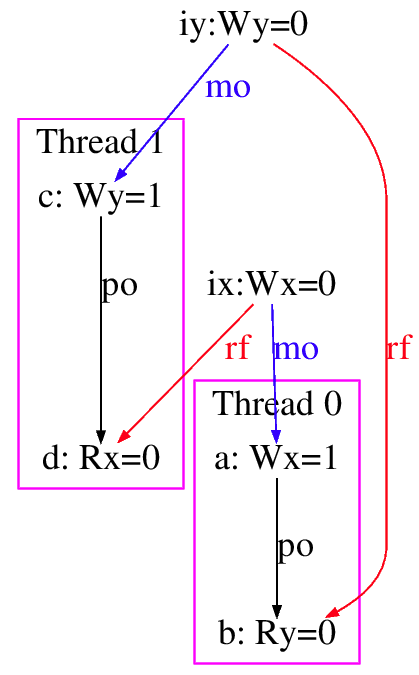
\includegraphics[width=4.5cm]{exec}
	\end{figure}

\end{frame}

\begin{frame}{RC11 : events}

	\begin{itemize}
	\item fences
	\item non atomic memory events
	\item atomic memory events annotated with a memory order
	\end{itemize}
	\vfill
	data race: when two events that aren't both atomic or both reads can access the same location at the same time.
	\vfill
	Data races cause unspecified behaviour.

\end{frame}

\begin{frame}{RC11 : properties}

	\vfill
	\begin{itemize}
	\item $\hb ; \eco ^?$ is irreflexive. \hfill (coherence)
	\item $\rmw \cap (\rb ; \mo) = \emptyset$. \hfill (atomicity)
	\item $\po \cup \rf$ is acyclic. \hfill (no-thin-air)
	\item $\psc$ is acyclic. \hfill (sequential-consistency)
	\end{itemize}
	\vfill

\end{frame}

\begin{frame}{Herd}
	\begin{figure}
	\centering
	{\fontsize{10pt}{0}
	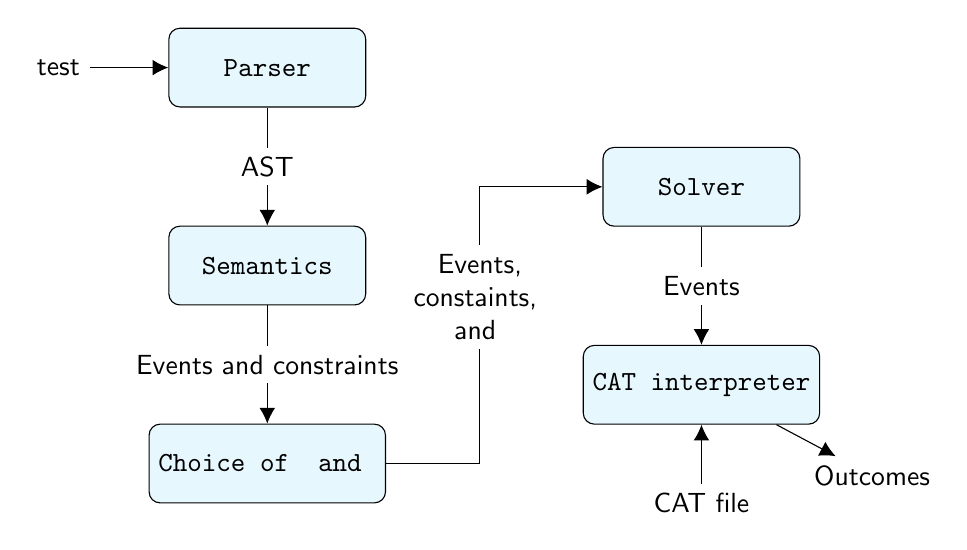
\begin{tikzpicture}[every node/.style={fill=white, font=\sffamily}, node distance=1.5cm, align=center]

	\node (start) [invisible] {test};
	\node (parser) [solid, right = 1cm of start] {Parser};
	\node (sem) [below = of parser, solid] {Semantics};
	\node (choice) [below = of sem, solid] {Choice of $\rf$ and $\mo$};
	\node (solver) [below right = 0.5cm and 3 of parser, solid] {Solver};
	\node (interp) [below = of solver, solid] {CAT interpreter};
	\node (end) [invisible, below right = 0.4cm and -0.2cm of interp] {Outcomes};
	\node (model) [invisible, below of = interp] {CAT file};
	
	\draw[->] (start) -- (parser);
	\draw[->] (parser) -- node {AST} (sem);
	\draw[->] (sem) -- node {Events and constraints} (choice);
	\draw[->] (choice) -| ++(2.7,1) |- node[text width=2cm, minimum size = 0.1cm, yshift=-1.4cm] {Events, constaints, $\mo$ and $\rf$} (solver);
	\draw[->] (solver) -- node {Events} (interp);
	\draw[->] (interp) -- (end);
	\draw[->] (model) -- (interp);
	
	\end{tikzpicture}}
	\end{figure}

\end{frame}

\begin{frame}{Herd}

	\vfill
	Generates every combination of $\rf$ and $\mo$, this is computationally expensive.
	\vfill
	Dealing with large sets of executions is a common problem for model checkers.
	\vfill
	\vfill
	Solution : a stateless algorithm that avoids this.

\end{frame}

\begin{frame}{The stateless algorithm}

	All RC11 properties but SC are monotonous.
	\vfill
	Work recursively :
	\begin{itemize}
	\item start with a consistent partial execution.
	
	\item add an event 
	
	\item generate all possible consistent partial executions.
	
	\item call the algorithm recursively on every generated execution
	\end{itemize}
	\vfill

\end{frame}

\begin{frame}{How the stateless algorithm works}

	\begin{figure}
	\centering
	{\fontsize{10pt}{0}
	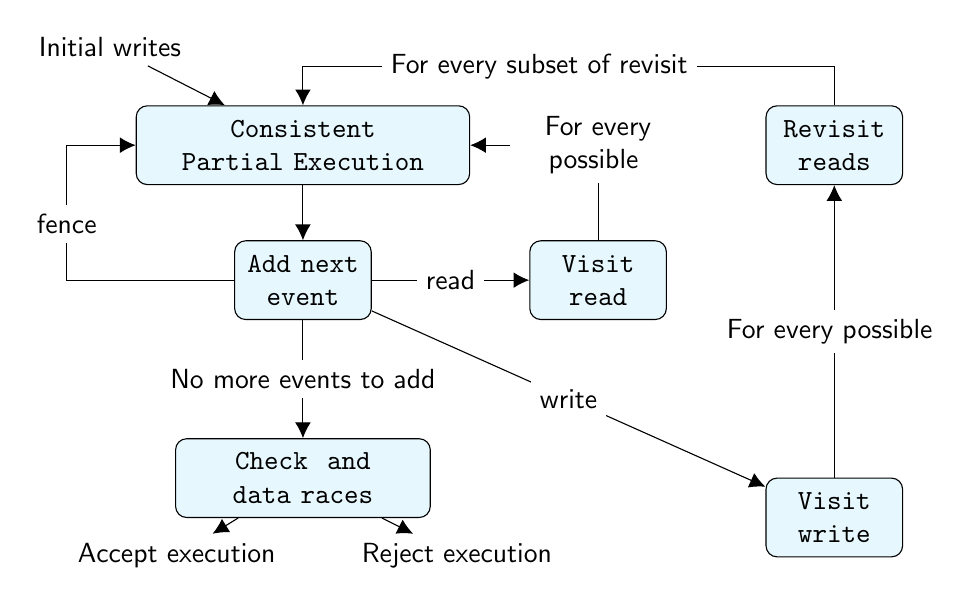
\begin{tikzpicture}[every node/.style={fill=white, font=\sffamily}, node distance=1.5cm, align=center, minimum width = 0]
	
	\node (cpe) [solid, text width = 4cm]{Consistent Partial Execution};
	\node (add) [solid, below = 0.7cm of cpe, text width = 1.5cm, minimum width = 0] {Add next event};
	\node (read) [solid, right = 2cm of add, text width = 1.5cm, minimum width = 0] {Visit read};
	\node (write) [solid, below right = 2cm and 5cm of add, text width = 1.5cm, minimum width = 0] {Visit write};
	\node (revisit) [solid, right = 3.75cm of cpe, text width = 1.5cm, minimum width = 0] {Revisit reads};
	\node (done) [solid, below = of add, text width = 3cm] {Check $\psc$ and data races};
	\node (in) [invisible, above left = 0.5cm and -0.7cm of cpe] {Initial writes};
	\node (accept) [invisible, below left = 0.2cm and -1.4cm of done] {Accept execution};
	\node (reject) [invisible, below right = 0.2cm and -1cm of done] {Reject execution};
	
	
	\draw[->] (cpe) -- (add);
	\draw[->] (add) -- node {read} (read);
	\draw[->] (add) -- node {write} (write);
	\draw[->] (add) -- node {No more events to add} (done);
	\draw[->] (add) -| ++(-3cm,0) |- node[yshift=-1cm] {fence} (cpe);
	\draw[->] (read) |- node[text width = 2cm] {For every possible $\rf$} (cpe);
	\draw[->] (write) -- node {For every possible $\mo$} (revisit);
	\draw[->] (revisit) |- ++(0,1cm) -| node[xshift = 3cm] {For every subset of revisit} (cpe);
	\draw[->] (in) -- (cpe);
	\draw[->] (done) -- (accept);
	\draw[->] (done) -- (reject);
	
	\end{tikzpicture}}
	
	\end{figure}	 

\end{frame}

\begin{frame}{Differences between the reference and my implementation}

	Herd generates a set of events and constraints per possible path.
	
	This means that some partial executions get computed more than once.
	\vfill
	This also means that some parts of the reference algorithm aren't relevant to herd.

\end{frame}

\begin{frame}{Work done}

	So far, I have :
	\begin{itemize}
		\item implemented RC11 in CAT.
		\item implemented the RC11 check directly into herd.
		\item started but not quite finished implementing the stateless algorithm in herd.
	\end{itemize}
	\vfill
	Should time allow it, I will try implementing smt based rc11 model checking techniques as well.

\end{frame}

\end{document}